\قسمت{بررسی تاثیر استفاده از انتگرال فازی در بهبود دانش جمعی}
همانطور که در بخش‌های قبلی دیدیم، استفاده از توابع $g(\cdot)$ مختلف در انتگرال فازی نتایج روش پیشنهادی موثر واقع شده‌اند و در نهایت با استفاده از تابع $\text{Const-One}$ که باعث می‌شود انتگرال فازی به یک عملگر بیشینه‌گیری تبدیل شود و بطور حریصانه در هر مرحله‌ی به اشتراک‌گذاری دانش، فقط دانش عاملی را به عنوان دانش جمعی خروجی الگوریتم در نظر بگیرد؛ در این بخش می‌خواهیم این موضوع را بررسی کنیم که تاثیر انتگرال فازی در بهبود دانش جمعی چگونه می‌باشد؟ به عنوان مثال آیا همیشه استفاده از انتگرال فازی در بهبود دانش جمعی موثر واقع است؟

در پاسخ به این سوالات، ما روش SEP را با این‌بار با استفاده از انتگرال فازی مورد آزمون قرار دادیم که همانطور که در شکل‌ \ref{fig:sep_maze_fci} مشاهده می‌کنیم وقتی در روش SEP بجای میانگین وزنی (روش پیشنهادی \مق{SEP}) از انتگرال فازی با توابع معرفی شده در الگوریتم‌های \ref{alg:g:max} تا \ref{alg:g:k-mean} استفاده کنیم برعکس نتایج بدست آمده خروجی انتگرال فازی کیفیت و سرعت یادگیری را بهبود نبخشید -- گرچه ممکن است در صورت تعریف توابع $g(\cdot)$ دیگر نتایج بهتری تولید کند؛ ولی در صورتی که از الگوریتم \ref{alg:g:const-one} استفاده کنیم بهترین نتیجه‌ی ممکن را می‌گیریم (همانند آنچه که در نتایج روش پیشنهادی نیز دیدیم).

\begin{figure}
\centering
\caption{تاثیر استفاده از انتگرال فازی در روش SEP بروی کیفیت و سرعت یادگیری در محیط پلکان مارپیچ}\label{fig:sep_maze_fci}
\begin{tabular}{*1c}
\subf{\includegraphics[width=.8\textwidth]{boltzmann/pref/sep/env/maze/fci-check.png}}
     {الف - استفاده از انتگرال فازی در روش SEP در محیط پلکان مارپیچ}
\\
\subf{\includegraphics[width=.8\textwidth]{boltzmann/pref/sep/env/prey/fci-check.png}}
{ب - استفاده از انتگرال فازی در روش SEP در محیط صید و صیاد}
\end{tabular}
\end{figure}